\subsection*{Technical Details}

\begin{sidewaysfigure}[!]
  \centering
  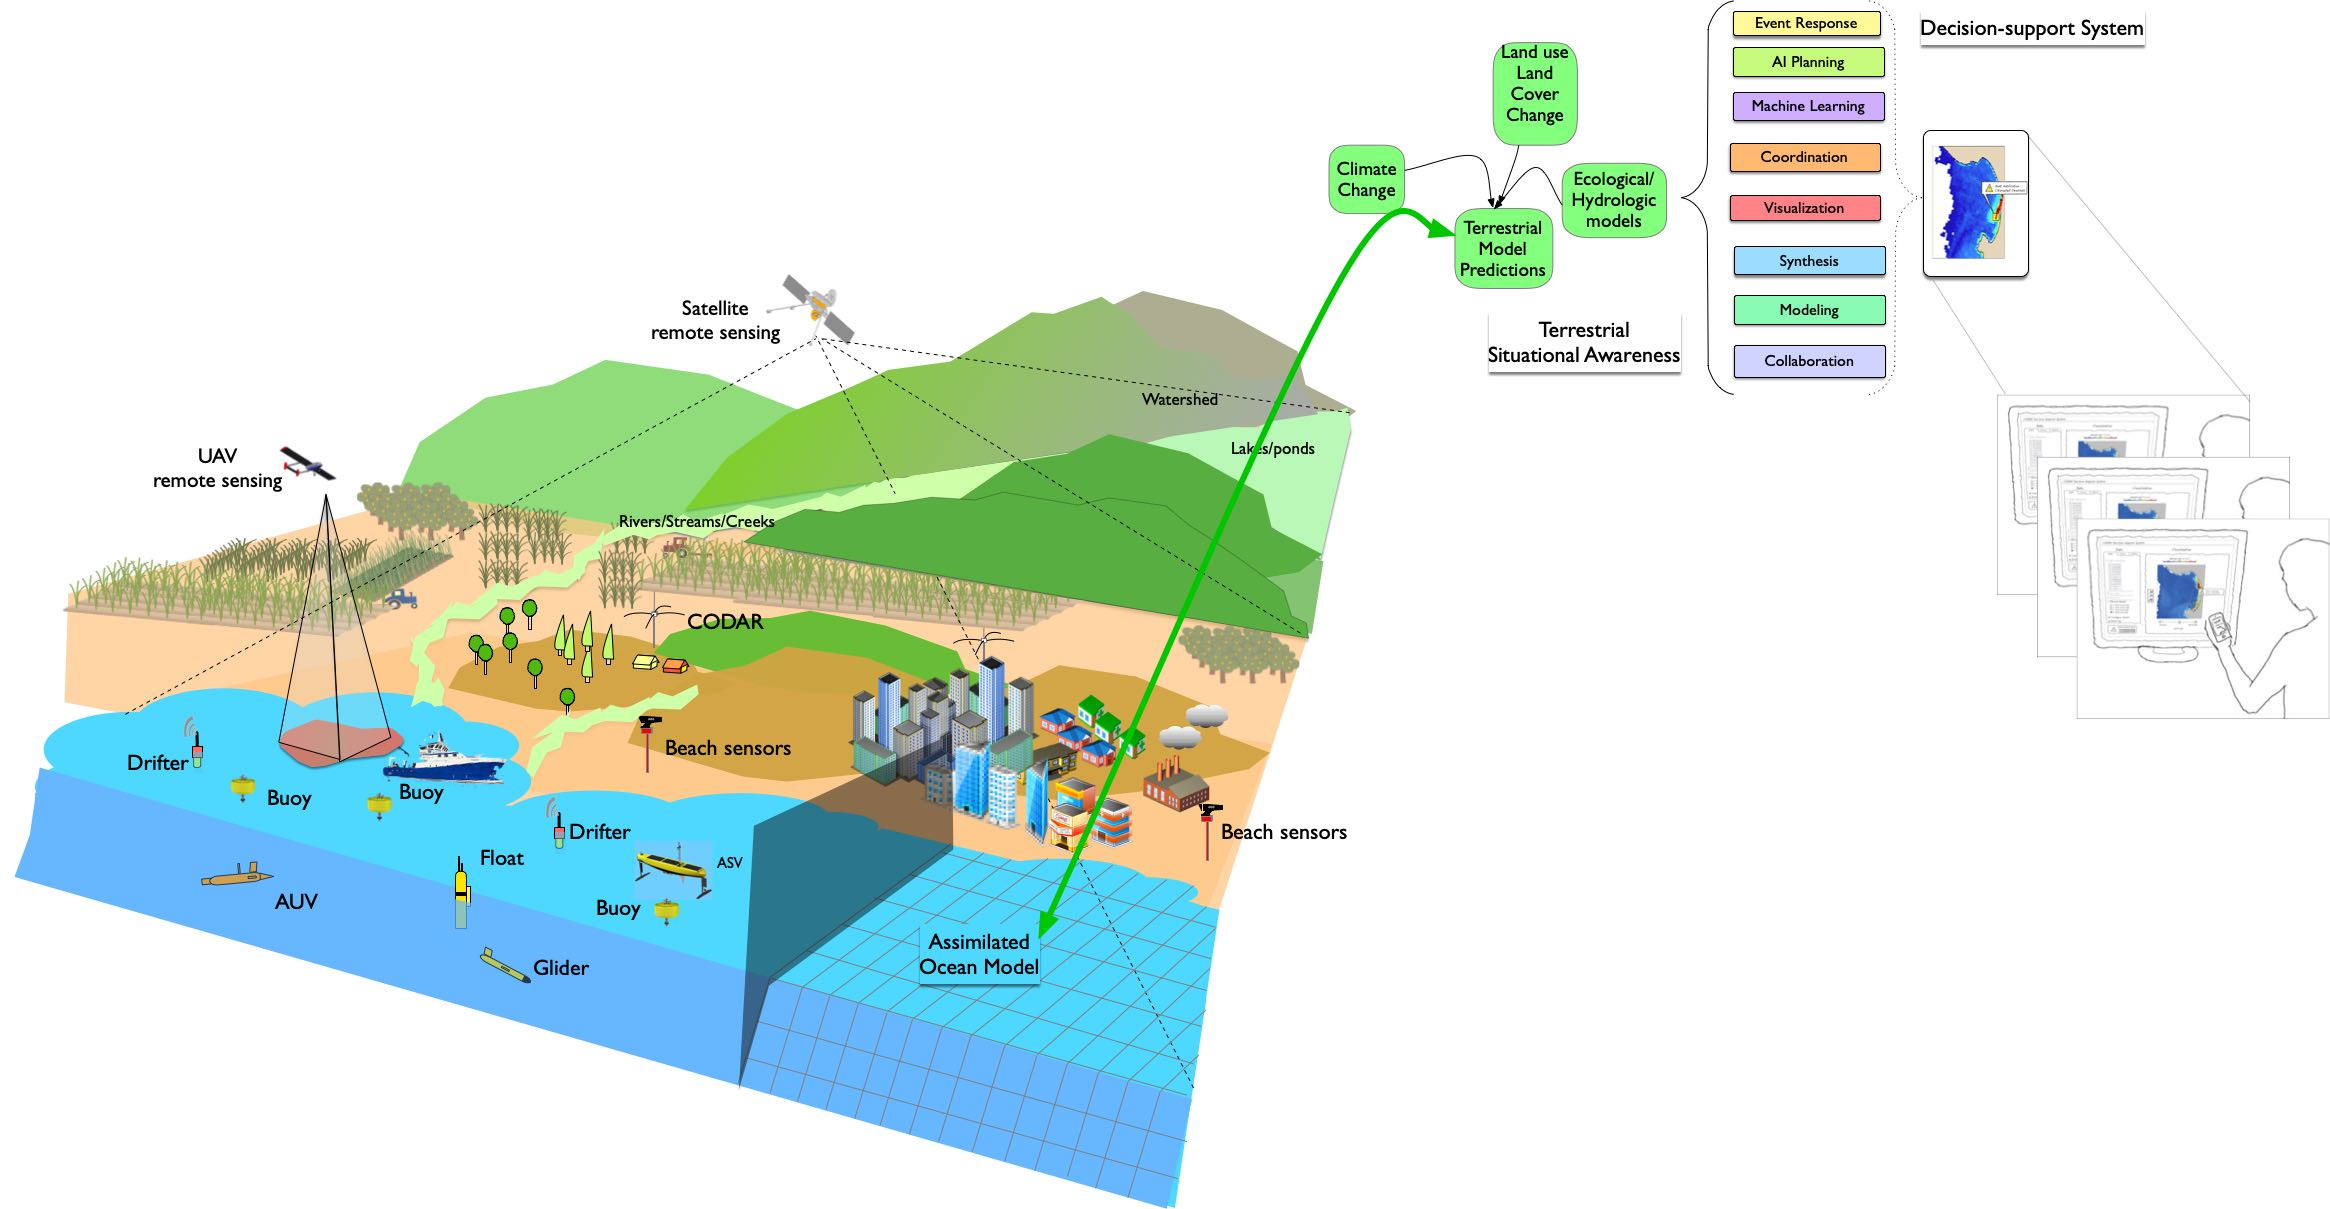
\includegraphics[scale=0.30]{fig/Coastal-connect.jpg}
  \caption{Networked space, aerial, surface, terrestrial and underwater
    platforms can gather high-resolution data in space and time to
    increase the predictive power of ocean driven extreme events.}
  \label{fig:coastal-res}
\end{sidewaysfigure}

\subsubsection*{Overview}

Extreme events are on the increase, impacting not only coastal
communities, but those deep within terrestrial domains, across the
world. Within the US, the typical Fall season has oceanic events
impacting coastal regions including flooding and extreme surf events
leading to large scale destruction of property and loss of lives. With
the increases in sea surface temperature and consequent energy stored
in the upper ocean, the atmospheric-ocean surface interaction has
become the driver for high intensity hurricanes well offshore and
tornadoes well inshore, as a means for captive energy transport. These
too have shown to lead to substantial and destructive impacts to human
lives and property. 

The oceans therefore are increasingly a key driver for such extreme
events. Our need to protect lives and property inland, including
coastal regions and urban centers at the block level, is increasingly
driven by what we need to know about the state of the oceans. This
form of interconnection is also related to how we are prepared for
natural emergencies which are endemic these days.

\subsubsection*{Sensor Network}


\begin{wrapfigure}{!r}{0.45\textwidth}
  \centering
  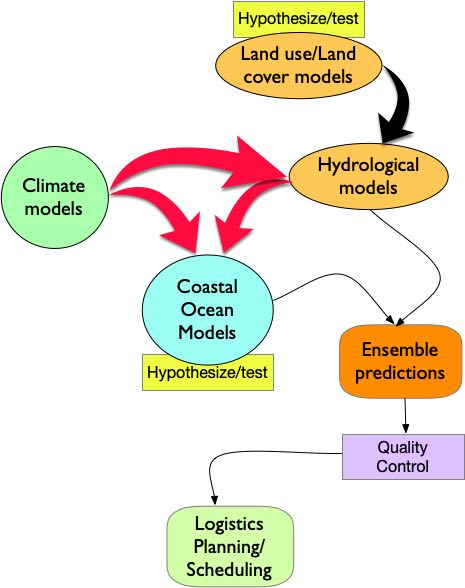
\includegraphics[scale=0.30]{fig/process.jpg}
  \caption{A range of predictive models will need to generate a QC-ed
    output, which can then be run into a logistics planning/scheduling
    engine during 'what-if' analyses.}
  \label{fig:process}
\end{wrapfigure}

We propose an \emph{integrative} effort to couple riverine/estuarine,
hydrologic and ocean models, driven by an ensemble of static and
mobile sensors on autonomous robotic platforms which sense-plan-act to
reduce modeling uncertainty, provide high resolution data and
consequent predictions, doing so with timeliness. An ensemble
prediction then combine these model outputs, to generate a final
prediction which must be quality-controlled (QC-ed) to drive a
logistics planning/scheduling tool. In so doing, a stakeholder can
seamlessly use the hypothesize/test function as a way to generate a
range of scenarios, which will automatically be incorporated into an
ocean or land use model. This would then trigger a novel prediction,
available for potential logistics planning (Fig. \ref{fig:process}).

To do so, we believe, networked mobile autonomous systems with an
AI-driven 'back end' software infrastructure can provide highly
effective ways to make not only 'what if' analyses for a range of
stakeholders for disaster management, but also provide targeted ways
in which the impact to various parts of the geography can be
estimated. Data is critical, especially for dynamically evolving
environmental conditions. To gather it, we need multiple ways and
multiple variables for measurement necessitating the need for a range
of platforms. Robotic platforms making in-situ measurements across the
aerial, surface and underwater domains (Fig. \ref{fig:coastal-res})
feed a range of calibrated sensor data to ocean models, which are
coupled with the local diurnal tidal cycle and estuarine predictions
can then make detailed predictions about the onset of offshore
climate's impact on the landmass. Predictions from shore then can be
propagated into a terrestrial/hydrological model to measure the impact
of high winds, tidal surges and hurricanes on inland communities.


\subsubsection*{System Modeling}

Typically land use, hydrological and ocean models are distinct,
derived and worked on in distinct communities with varied expertise.
We advocate an integrative approach to combine these methods in ways
that can provide decision-makers a valuable new tool which can be
portable across domains and demonstrate the power of integration.

Land use and hydrologic models can be integrated with ocean models to understand the complex interactions between the ocean environment and land and water dynamics. Land use models, such as the Community Land Model (CLM) simulate land and vegetation responses to climate and other environmental changes. They are capable of estimating crop dynamics, urban climate, land cover change, among others. Models such as CLM also simulate the hydrologic cycle. For more detailed estimations of flooding, drought or other climate impacts on water systems, more detailed hydrologic models can be used. These models can be deployed at sub-urban to national scales to understand where flooding may occur in responses to extreme precipitation events, or how drought can affect water supply across arid regions.


\begin{wrapfigure}{!r}{0.45\textwidth}
  \centering
  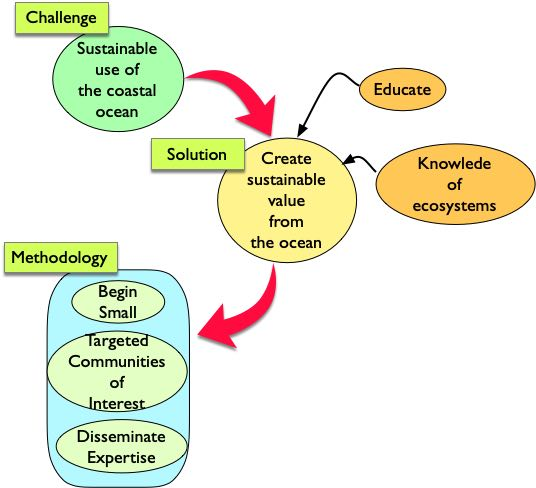
\includegraphics[scale=0.40]{fig/Ericeira-method.jpg}
  \caption{Using a mix of models integrated between coastal, terrestrial
    and land use methods could enhance sustainable ways of exploiting
    resources, both terrestrial and oceanic.}
  \label{fig:method}
\end{wrapfigure}


\subsubsection*{Integration}

Logistical considerations related to where (and when) emergency
management resources can then make targeted assessments of support
functions at precise locations and times. Legacy systems for disaster
preparedness could be interfaced with the ensemble
predictions. However, the power of Machine Learning methods could be
applied to ensure the right use of assets in ways that impact
assessments can be qualitatively measured to have the right assets at
the right place and time. 

This interconnected system-of-systems could used in a range of ways,
including in real-time disaster assessment, assessments of property
damage with aerial and space based remote sensing using before/after
imagery in targeted ways, as well as for multiple Monte-Carlo based
gaming assessments to hypothesize a range of diaster management
scenarios. These in turn could lead to Machine Learning based approaches
on high probability areas where logistical storage could be berthed in
order to have the maximum impact in terms of delivery and help to
victims of such natural events.

At a larger scale, climate models can be incrementally coupled into
such an ensemble of models to add to the longer term predictive power
(Fig. \ref{fig:coastal-res}) as a way to enhance estimation over
extreme cases. Not only will such an approach be critical for purposes
of resiliency, it will provide a range of stakeholder options on how
to make informed assessments on \emph{where} and \emph{when} to
provide support while enhancing sustainable use of resources both
coastal and terrestrial (Fig: \ref{fig:method}).

